\section{Event identification}
During production, runs were taken in batches of three, one each with \snTwelve,
\snFour, and the blank samples. Because the distance to each time-of-flight detector
was already measured, the time-of-flight for elastically-scattered neutrons could
be directly calculated and used to determine delay from electronics and cabling.
The timestamp of each event was thus adjusted by a fixed amount
so that the first peak of the neutron spectrum aligned the expected
time-of-flight. Next, background $\gamma$-ray events were separated from relevant
neutron events by a pulse-shape discrimination analysis, shown in Fig. \ref{PHPSDPlot}.

\begin{figure}[ht]
    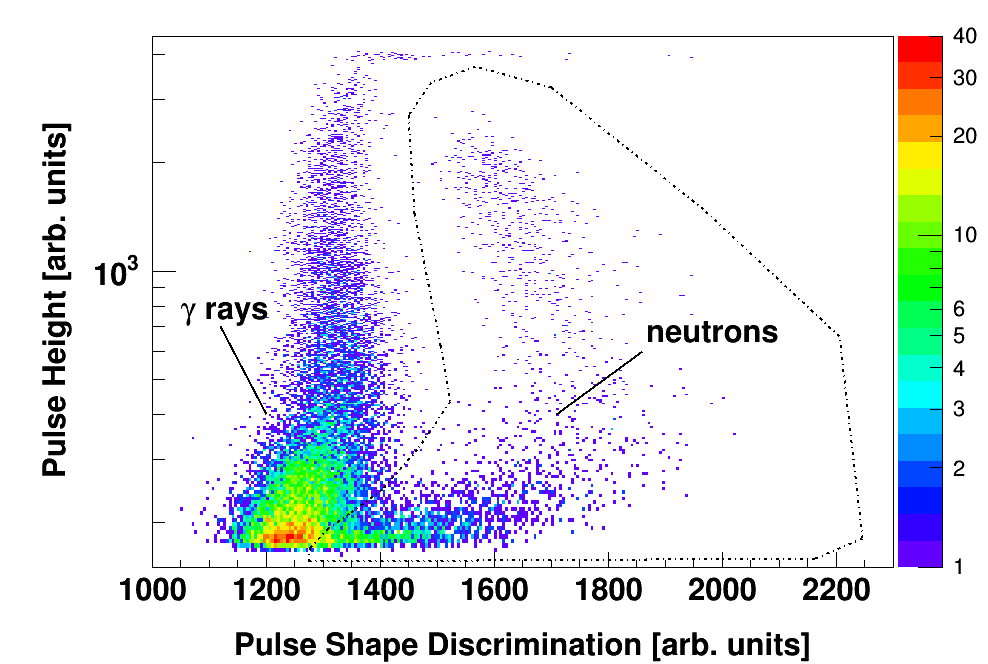
\includegraphics[width=0.9\textwidth]{figures/PHPSDPlot.png}
    \caption[Event pulse height (PH) vs. pulse-shape-discrimination (PSD) for
    a typical run]
    {
        Event pulse height (PH) vs. pulse-shape-discrimination (PSD) for
        a typical run. A gate (dashed line) isolates neutron events, which are
        used for subsequent analysis. At low pulse heights, the PSD output from the
        MPD-4 module is non-linear, making neutron-$\gamma$-ray separation more difficult
        (bottom-left of the figure).
    }
    \label{PHPSDPlot}
\end{figure}

Neutron events surviving this PSD gating are shown for a few typical runs in Fig. 
\ref{tiledRunData}. The first and second subfigures in the left column of the figure are from 
the same detector and arm angle, but the first is from a blank-sample run and
the second is from a \snFour sample-run. In each subfigure, the expected location
of the time-of-flight for elastic scattering on \snFour is marked with a dark blue arrow,
and the approximate FWTM time
resolution of the detector is marked with blue dashed lines. The expected
location of the time-of-flight peak for elastic scattering on atmospheric
N$_{2}$ is marked with a green arrow. The additional counts in the 55-57 ns region in
the second subfigure (compared to the first) are from elastic scattering on
\snFour. Energy-dependent detector efficiencies for each detector were provided by TUNL
and are shown above each histogram. For clarity, these efficiencies are plotted
relative to the efficiency of at the elastically-scattered neutron energy.

\begin{figure}[ht]
    \centering
    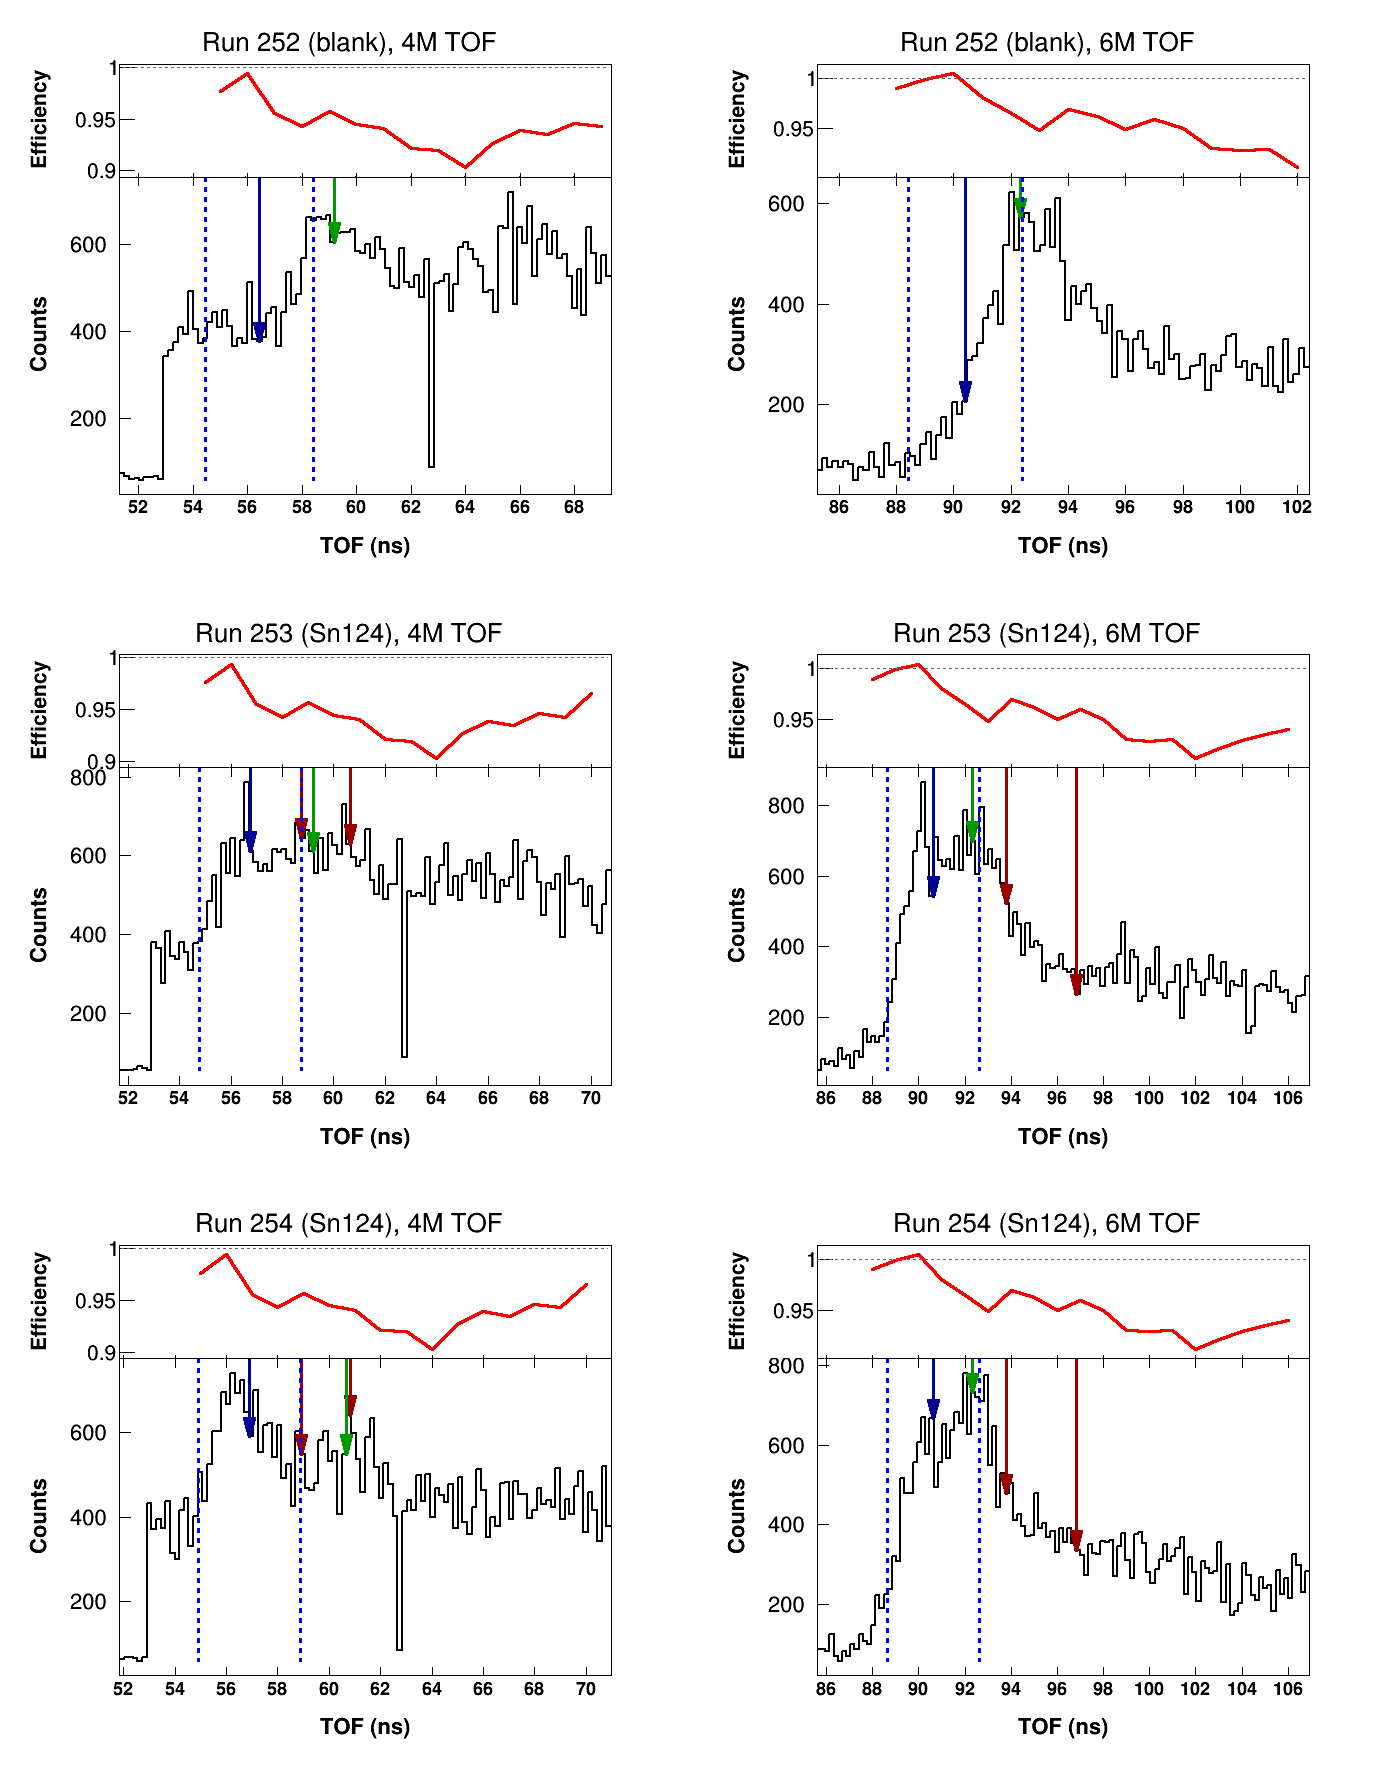
\includegraphics[width=0.9\textwidth]{figures/tiledRunData.png}
    \caption{Histograms from typical runs showing neutron elastic scattering peak} 
    {
        Neutron-event histograms for three typical runs, one with the blank
        sample and two with the \snFour sample.
        The expected location of the \snFour elastic scattering peak (dark blue arrow)
        and first two inelastic scattering peaks (light blue arrows) show an
        increased number of counts when the sample is in-beam (runs 253 and
        254). For reference, the expected location of the nitrogen elastic scattering
        peak is shown as green arrows and the expected location of the first- and
        second-inelastic scattering peaks for \snFour are shown as red arrows.
        The FWTM detector resolution is indicated by the blue dashed lines.
    }
    \label{tiledRunData}
\end{figure}

After scaling histogram counts by detector efficiency, histograms were
normalized by the total neutron flux
(i.e., total counts in the CMON detector for that run) and summed by detector
angle. Then, blank-run histograms
were subtracted from the isotopic-run histograms to yield the neutron scattering
events from the isotopic samples. Figure \ref{tiledAngleData} depicts the
results. As in the previous figure, dark blue arrows mark the anticipated
time-of-flight of the elastic scattering peak, green arrows mark elastic
scattering from atmospheric nitrogen, and blue dashed lines mark the anticipated
FWTM of the elastic scattering peak. Inelastic scattering peaks from the first and
second excited states samples are marked with light blue
arrows. For the 4M detector and at forward angles for both detectors, the elastic and first 
inelastic scattering peaks are closer in time and cannot be cleanly resolved. Measurements in this
kinematic regime are the most challenging as the increased overlap between
these peaks increases the uncertainty of the number of counts in the elastic
peak. We fit the amplitudes of two Gaussian distributions to the elastic and
first-inelastic peaks while fixing
the $\mu$ and $\sigma$ of each Gaussian according to our detector resolution and
the expected time-of-flight. Then, we integrated the first Gaussian to recover the
number of counts in the elastic peak.

\begin{figure}[ht]
    \centering
    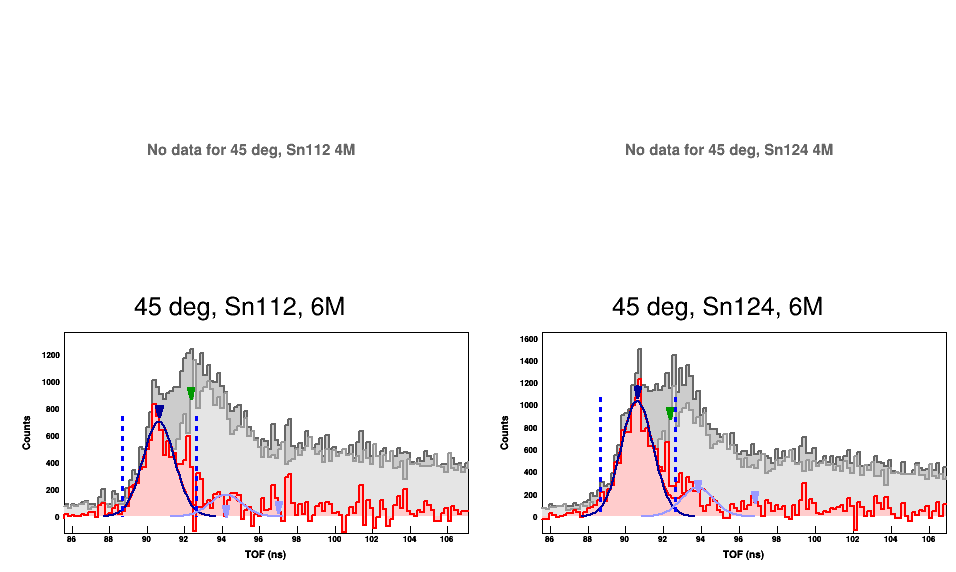
\includegraphics[width = 0.9\textwidth]{figures/tiledAngleData.png}
    \caption[Scaled event histograms showing neutron elastic scattering peak]
    {
        Scaled event histograms showing neutron elastic scattering peak. The
        neutron event histograms for isotopic-sample runs (dark gray),
        blank-sample runs (light gray), and the difference (in red) are plotted.
        The dark blue arrows indicate the expected location of the elastic scattering
        peaks on \snTwelveFour, and the light blue arrows indicate the first-
        and second-excited inelastic scattering peaks on \snTwelveFour. The
        green arrows indicate the expected location of the elastic scattering
        peaks on atmospheric N$_{2}$. A double-Gaussian function was fit to the
        subtracted histogram and the results of the fit drawn in dark
        blue (elastic peak) and light blue (first-inelastic peak).
    }
        \label{tiledAngleData}
\end{figure}

\section{Normalization}
To normalize the cross sections, the absolute neutron flux must be known.
To determine the absolute neutron flux, a few initial reference runs were taken using a graphite,
a polyethylene, and a blank sample. Events from one batch of these runs are
histogrammed in Fig. \ref{polyethyleneRef} for the 4M and 6M detectors.
The same conventions from Fig.
\ref{tiledAngleData} are used, except that now the light blue arrows correspond to
the elastic and first-excited peaks of C. The dark gray histogram (back
histogram layer) shows the elastic and first-excited peaks of C
and also a broad peak from elastic scattering on H. After scaling for the number
of moles in the graphite and polyethylene samples, stoichiometry, and neutron
flux, the graphite spectrum (light gray, middle histogram later) is subtracted from the polyethylene
spectrum, yielding neutron events from elastic scattering on protons (area of
the red histogram between the blue dashed lines). Given the
well-established n(p,p)n cross section, the ratio of absolute neutron flux to
the number of CMON counts can be calculated:

\begin{equation}
\end{equation}

\noindent
We used the Scattering Analysis Interactive Database (SAID) code \cite{SAIDCode}
to generate
the proton-neutron elastic scattering cross sections needed in the above
equation. This flux-to-monitor ratio was then used to normalize the \snTwelveFour
results.

\begin{figure}
    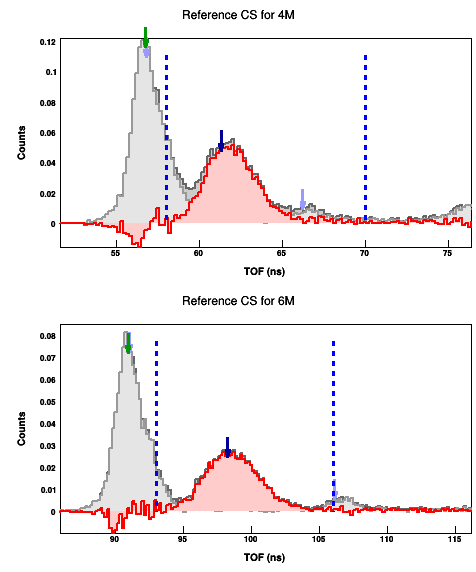
\includegraphics[width = 0.9\textwidth]{figures/polyethyleneRef.png}
    \caption[Reference runs of neutron scattering on C and (CH$_{2}$)$_{n}$]
    {
        Reference runs of neutron scattering on C and (CH$_{2}$)$_{n}$
        The (CH$_{2}$)$_{n}$ run (back histogram, in dark gray) and C run
        (middle histogram, in light gray) are scaled by beam flux and number of
        atoms in each sample. Their difference (front histogram, in red) shows a
        broad peak corresponding to neutron-proton elastic scattering. The
        expected time-of-flight for this peak is shown by the blue arrow. The light blue arrows 
        indicate the expected position of the elastic and first-excited peaks
        from scattering on C. The green arrow indicates the expected position of
        the elastic peak from scattering on atmospheric N$_{2}$.
    }
    \label{polyethyleneRef}
\end{figure}

\section{Cross Section Calculation}

\begin{equation}
\end{equation}

\section{Finite Size Corrections}
In an idealized differential cross section measurement, the sample and neutron
detectors can be treated as point objects. In reality, the neutron beam,
samples, and detectors occupy a finite size, leading to so-called finite-size
effects that distort the measured cross sections. The experimenter is responsible
for applying appropriate corrections so that reported results are size- and
apparatus-independent.

The finite-size analysis of Guss et al. for
their neutron \el\ measurements on $^{116,120}$Sn is given in great detail in
\cite{GussPhDThesis}. Monte carlo simulations are used to generate a correction
for the uncertainty in neutron scattering path, multiple-scattering
in the samples, and flux attenuation in the sample \ref{GussFiniteSizeEffect},
all of which they found to be important corrections on the order of 1-10\%.
However, their isotopic samples were an order of magnitude larger than our
samples (42.59 g and 44.73 g for their \snSixteen and \snTwenty samples,
respectively), dramatically increasing the finite-size effects. Given the small amount of sample 
material in our measurement (4.97 g and 5.55 g for our \snTwelve and \snFour
samples, respectively), the finite size corrections required were much
smaller. The geometric finite-size correction from angular uncertainty in the
scattered neutron flight path is mostly a function of the sample volume,
not the number of sample atoms. Thus the angular uncertainty of the neutron
scattering path is approximately half as large as that calculated by Guss et al,
as our sample diameters and radii were smaller than the Guss et al. samples
by roughly a factor of two. The multiple-scattering and flux attenuation
effects, however, are proportional to the number of atoms
encountered by neutrons after their first scattering event. Because the number
of atoms in our samples was an order of magnitude smaller than those of Guss et
al., these latter finite size corrections were anticipated to be approximately
an order of magnitude smaller and thus have a negligible effect on our results.
The same could not be said of the geometric finite-size effects \textit{a
priori}, so a simulation was prepared and the details are presented below.

Because the samples and angular detectors are not point-like, the exact
path of elastically-scattered neutrons is subject to a small degree of angular
uncertainty. The effect of this uncertainty is that in the measured cross
sections, the maxima and minima are "washed out" compared to the true cross
section, especially in regions where the cross section varies rapidly compared
to the angular uncertainty. To assess the magnitude of this effect, a 
simulation was prepared in which a uniform beam of neutrons
impinged on the sample volume and was scattered into the time-of-flight
detectors [insert figure reference].
The input cross section, used to distribute neutrons in the simulation, was
taken as the raw cross section from our measurement. Then, a new, "output"
cross section was calculated based on the detector hits in the simulation. The
output cross section is thus a weighted convolution of the input cross section
with the size uncertainty of the samples and detectors.
A comparison between the input and output cross
sections shows this geometric finite-size effect is quite small in our case, much smaller
than other sources of measurement error. Nevertheless, our results below include an
angle-dependent correction calculated from this simulation. The small size of
the geometric effect gives us confidence that the multiple-scattering and flux
attenuation corrections mentioned previously can be neglected without impacting
our results.

For simplicity, the simulation was purely geometric - no nuclear physics or
energy-dependence was included. For each Monte Carlo iteration, the beam was
assumed to uniformly illuminate
the sample from one direction so that the scattering vertex was randomly
distributed within the sample volume. At the scattering vertex, a neutron
trajectory was selected by randomly sampling an "input cross section" as a
probability mass function, thus weighting the neutron scattering angles by the
input cross section.  Once the trajectory was known, each detector's location
and orientation was used to calculate the point of intersection in the plane of each detector. If the
intersection fell within the detector's face, the detector registered a hit.
Finally, the "output cross section" (that is, the result of the simulation)
was calculated by normalizing the number of counts registered in each detector
over the total number of iterations and the fraction of the total solid angle
subtended by said detector.

The results of the simulation are visible in Fig. [X]. For the sample and
detector sizes actually used in the experiment, the deviation between the input
and output cross sections is <1\% over all angles. When exaggerated sizes for the
sample and detectors are used, the finite-size effect is visible as a "washing
out" of minima and maxima in regions where the cross section varies rapidly with
angle. To calculate a correction factor for our results, we divided the simulation's
input cross section by the output cross section for each angle and multiplied our
experimental results by this factor. In principle, this procedure to generate
the correction should be repeated iteratively because the correction changes the input distribution 
used for the simulation itself, but in practice the correction is so small
that no further iteration is required.

\section{Results}
\subsection{\snTwelveFour\ \el\ at 11 MeV}
Absolute cross sections 

\begin{figure}
    \begin{center}
        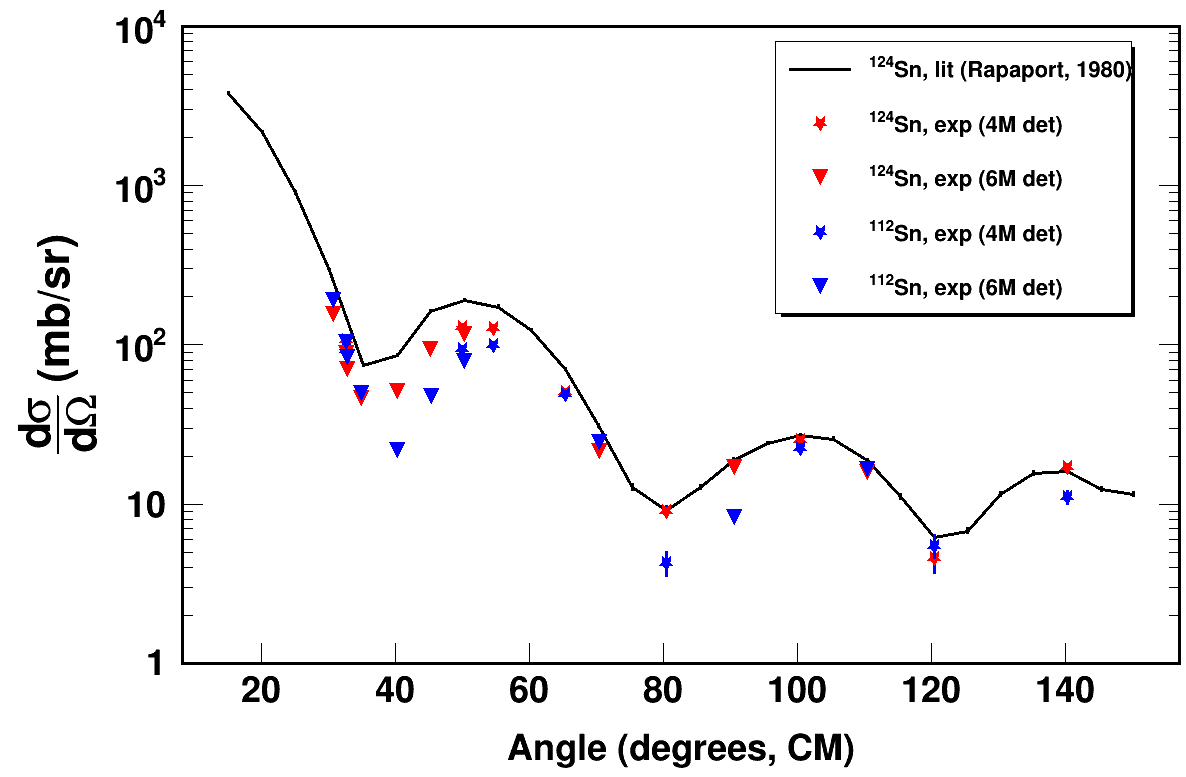
\includegraphics[width = 0.9\textwidth]{figures/neutronECS_Sn_11MeV.png}
        \caption{Neutron \el cross sections on $^{112,124}$Sn at 11
    MeV: our results and literature data}
    \label{SnECS_11MeV}
\end{center}
\end{figure}

\subsection{\snTwelveFour\ \el\ at 17 MeV}

\begin{figure}
    \begin{center}
        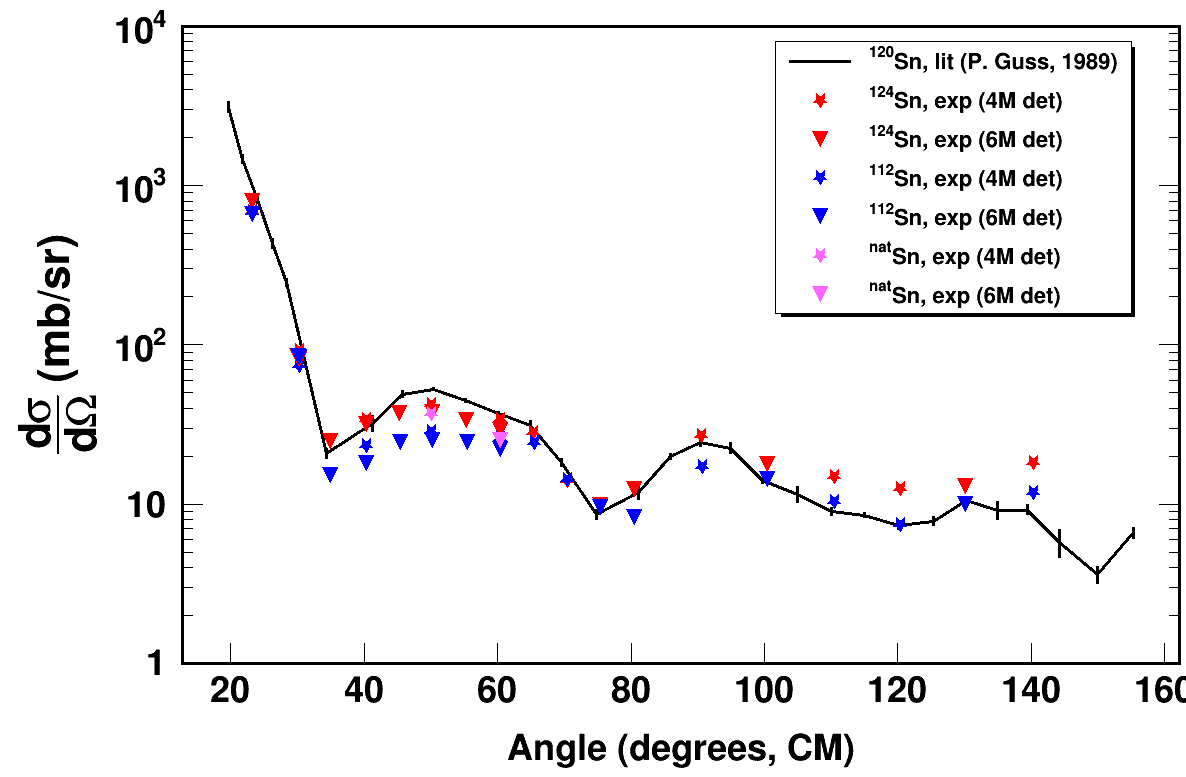
\includegraphics[width = 0.9\textwidth]{figures/neutronECS_Sn_17MeV.png}
        \caption{Neutron \el cross sections on $^{112,nat,124}$Sn at 17
    MeV: our results and literature data} \label{SnECS_17MeV}
\end{center}
\end{figure}

\afterpage{\clearpage}
